\documentclass[11pt,a4paper]{article}
\usepackage[spanish,es-nodecimaldot]{babel}	% Utilizar español
\usepackage[utf8]{inputenc}					% Caracteres UTF-8
\usepackage{graphicx}						% Imagenes
\PassOptionsToPackage{hyphens}{url}\usepackage[hidelinks]{hyperref}			% Poner enlaces sin marcarlos en rojo
\usepackage{fancyhdr}						% Modificar encabezados y pies de pagina
\usepackage{float}							% Insertar figuras
\usepackage[textwidth=390pt]{geometry}		% Anchura de la pagina
\usepackage[nottoc]{tocbibind}				% Referencias (no incluir num pagina indice en Indice)
\usepackage{enumitem}						% Permitir enumerate con distintos simbolos
\usepackage[T1]{fontenc}					% Usar textsc en sections
\usepackage{amsmath}						% Símbolos matemáticos
\usepackage{algpseudocode}
\usepackage{algorithm}

% no accents in math operators
\unaccentedoperators

% Comando para poner el nombre de la asignatura
\newcommand{\asignatura}{Aprendizaje Automático}
\newcommand{\autor}{Vladislav Nikolov Vasilev}

% Comandos utilies
\newcommand{\answer}{\noindent\textbf{Solución}}
\newcommand{\ein}{E$_{in}$}
\newcommand{\eout}{E$_{out}$}
\newcommand{\addtoc}[1]{\addcontentsline{toc}{section}{#1}}

% Configuracion de encabezados y pies de pagina
\pagestyle{fancy}
\lhead{\autor{}}
\rhead{\asignatura{}}
\lfoot{Grado en Ingeniería Informática}
\cfoot{}
\rfoot{\thepage}
\renewcommand{\headrulewidth}{0.4pt}		% Linea cabeza de pagina
\renewcommand{\footrulewidth}{0.4pt}		% Linea pie de pagina

\begin{document}
\pagenumbering{gobble}

% Pagina de titulo
\begin{titlepage}

\begin{minipage}{\textwidth}

\centering

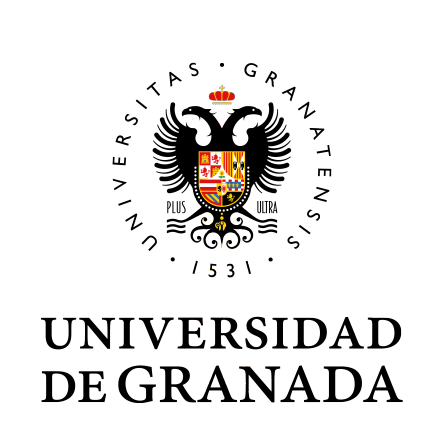
\includegraphics[scale=0.5]{img/ugr.png}\\

\textsc{\Large \asignatura{}\\[0.2cm]}
\textsc{GRADO EN INGENIERÍA INFORMÁTICA}\\[1cm]

\noindent\rule[-1ex]{\textwidth}{1pt}\\[1.5ex]
\textsc{{\Huge TRABAJO 3\\[0.5ex]}}
\textsc{{\Large Cuestiones de Teoría\\}}
\noindent\rule[-1ex]{\textwidth}{2pt}\\[3.5ex]

\end{minipage}

\vspace{0.5cm}

\begin{minipage}{\textwidth}

\centering

\textbf{Autor}\\ {\autor{}}\\[2.5ex]
\textbf{Rama}\\ {Computación y Sistemas Inteligentes}\\[2.5ex]
\vspace{0.3cm}


\includegraphics[scale=0.3]{img/etsiit.jpeg}

\vspace{0.7cm}
\textsc{Escuela Técnica Superior de Ingenierías Informática y de Telecomunicación}\\
\vspace{1cm}
\textsc{Curso 2018-2019}
\end{minipage}
\end{titlepage}

\pagenumbering{arabic}
\tableofcontents
\thispagestyle{empty}				% No usar estilo en la pagina de indice

\newpage

\setlength{\parskip}{1em}

\section*{Ejercicio 1}
\addtoc{Ejercicio 1}

\noindent ¿Podría considerarse Bagging como una técnica para estimar el error de predicción de un
modelo de aprendizaje? Diga si o no con argumentos. En caso afirmativo compárela con
validación cruzada.

\answer

Bagging se podría considerar como una técnica para estimar el error de predicción de un modelo de aprendizaje.
Esto se debe a que, a partir de una muestra, se eligen mediante \textit{bootstrapping} un número $B$ de conjuntos de entrenamiento
(es decir, conjuntos en los que hay datos con repetición), y se entrenan $B$ árboles con estas muestras de entrenamiento. El resto
de elementos de la muestra que no han sido escogidos para formar las muestras de entrenamiento se utilizan como test (es decir, para
cada árbol, se mira cuáles son los elementos de la muestra original que no han sido utilizados en el entrenamiento, y se escogen
posteriormente para hacer el test y obtener alguna métrica del error o de la precisión del árbol de manera individual). Finalmente,
se realiza la media con todos los resultados obtenidos para cada modelo.

Esto que se ha descrito en el párrafo anterior es muy parecido a lo que se hace con la validación cruzada. Ambos tienen una parte
de los datos con la que entrenan el modelo y una parte con la que obtienen alguna métrica sobre el modelo, para luego juntar todas
las métricas, hacer una media de éstas y obtener un valor que nos permita estimar el error de predicción del modelo.

Sin embargo, existen algunas diferencias:

\begin{itemize}[label=\textbullet]
	\item En la validación cruzada no hay datos repetidos ya que se hacen una serie de $k$ particiones disjuntas. En cambio, al
	utilizar \textit{bootstrapping} en Bagging, al escoger datos de la muestra con repetición, existen muy altas probabilidades
	de que se repita algún dato.
	\item En la validación cruzada se hacen $k$ particiones disjuntas y se prueba el mismo modelo con todas ellas agrupando
	los datos en una parte de training y una de test, haciendo que la partición de test sea cada vez diferente para las $k$
	particiones que se han creado. En cambio, con Bagging se entrenan una serie de $B$ modelos con un solo
	conjunto de entrenamiento cada uno y se prueba con un conjunto de test solo. Es decir, en vez de tener un único modelo que
	se va entrenando con cada una de las particiones de entrenamiento, se tienen $B$ modelos.
	\item En la validación cruzada se puede elegir qué parte de los datos estará en la parte de test, al poder elegir el tamaño
	de las particiones. En cambio, en Bagging aproximadamente 2/3 de los datos de la muestra original serán usados como training,
	mientras que aproximadamente el 1/3 restante será utilizado para test para cada modelo.
\end{itemize}

\section*{Ejercicio 2}
\addtoc{Ejercicio 2}

\noindent Considere que dispone de un conjunto de datos linealmente separable. Recuerde que una
vez establecido un orden sobre los datos, el algoritmo perceptron encuentra un hiperplano
separador interando sobre los datos y adaptando los pesos de acuerdo al algoritmo

\begin{algorithm}[H]
\caption{Perceptron}
\begin{algorithmic}[1]
\State \textbf{Entradas}: $(\mathbf{x}_i, y_i) = 1, \dots, n \; , \; w=0, \; k = 0$
\Repeat
	\State $k \gets (k + 1) \; \mod \; n$
	\If{$\text{sign}(y_i) \neq \text{sign}(\mathbf{w}^T\mathbf{x}_i)$}
		\State $\mathbf{w} \gets \mathbf{w} + y_i\mathbf{x}_i$
	\EndIf
\Until{todos los puntos bien clasificados}
\end{algorithmic}
\end{algorithm}

\noindent Modificar este pseudo-código para adaptarlo a un algoritmo simple de SVM, considerando
que en cada iteración adaptamos los pesos de acuerdo al caso peor clasificado de toda la
muestra. Justificar adecuadamente/matematicamente el resultado, mostrando que al final
del entrenamiento solo estaremos adaptando los vectores soporte.

\answer

\begin{algorithm}[H]
\caption{Perceptron-SVM}
\begin{algorithmic}
\State \textbf{Entradas}: $(x_i, y_i), i = 1, ..., n; \; w = 0, \; k = 0$
\Repeat
  \State $k \gets (k + 1) \mod n$
  \State $peor \gets$ peor clasificado
  \If{$y_{peor} \cdot w^t \cdot x_{peor} < 1$}
    \State $w \gets y_{peor} \cdot x_{peor}$
  \EndIf
\Until{convergencia}
\end{algorithmic}
\end{algorithm}

\section*{Ejercicio 3}
\addtoc{Ejercicio 3}

\noindent Considerar un modelo SVM y los siguientes datos de entrenamiento: Clase-1:$\lbrace (1,1),$
$(2,2),(2,0) \rbrace$, Clase-2:$\lbrace (0,0),(1,0),(0,1) \rbrace$

\begin{enumerate}[label=\textit{\alph*})]
	\item Dibujar los puntos y construir por inspección el vector de pesos para el hiperplano óptimo y el margen óptimo.
\end{enumerate}

\answer

Primero vamos a dibujar los puntos para ver como se ditribuyen en el espacio:

\begin{figure}[H]
\centering
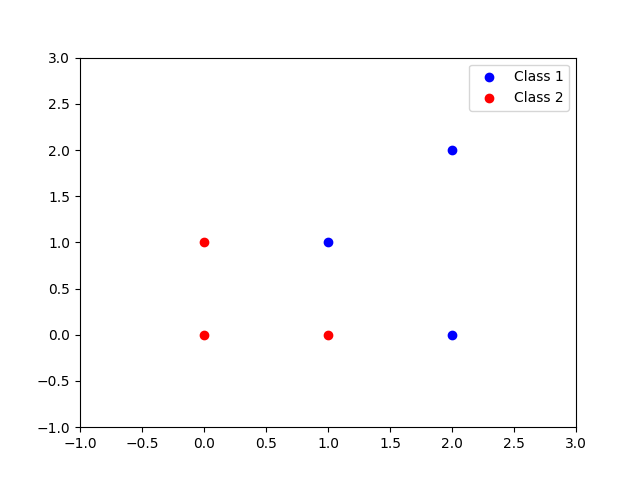
\includegraphics[scale=0.6]{img/points.png}
\caption{Dibujo con los puntos de las dos clases en el espacio.}
\end{figure}

Se puede ver claramente que los puntos de los dos clases son linealmente separables, ya que perfectamente se pueden separar mediante
un hiperplano que pase en medio de ellas.

Para intentar obtener un hiperplano óptimo, vamos a suponer que éste tiene que pasar entre los puntos de las dos clases que estén más
cerca entre sí (es decir, que tiene que pasar entre los vectores soporte). Estos puntos son, para la Clase-1, el $(1, 1)$ y el
$(2, 0)$, y para la Clase-2 son el $(0,1)$ y el $(1, 0)$. Por tanto, sabiendo que el hiperplano óptimo tiene que pasar entre estos
puntos, dejando la mayor cantidad de margen a cada lado, podemos suponer que pasará justo en el punto medio para cada par de puntos
que están a la misma altura y son de clases diferentes. Es decir, que para los puntos $(0, 1)$ y $(1, 1)$ (los cuáles son de
diferente clase), sabemos que seguramente ese hiperplano pasará por el $(0.5, 1)$. Para los dos puntos de abajo, sabiendo que tiene
que pasar entre los puntos $(0, 0)$ y $(1, 0)$, seguramente pasará por el punto $(1.5, 0)$, el cuál está justo en medio de los
dos anteriores. Esto se puede ver mejor en la siguiente imagen:

\begin{figure}[H]
\centering
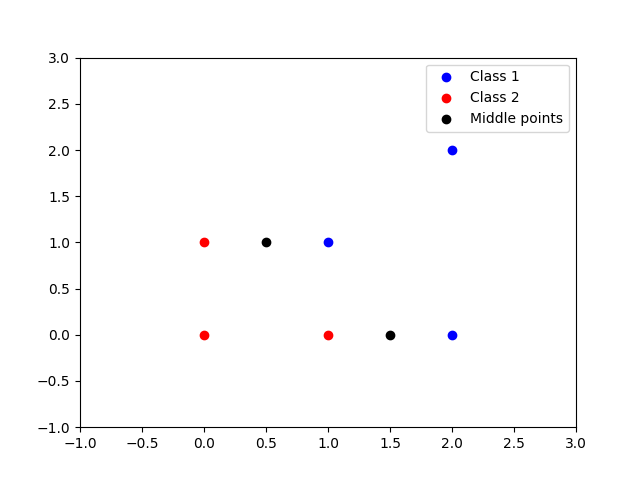
\includegraphics[scale=0.6]{img/middle.png}
\caption{Dibujo con los puntos medios entre los vectores soporte de las dos clases, representados en negro.}
\end{figure}

Ahora lo único que nos queda es obtener el hiperplano que separa las dos clases. Como ya sabemos los puntos por los que puede pasar,
lo único que tenemos que obtener es la recta que pasa por esos dos puntos. Para eso podemos partir de la ecuación de la recta, la cuál
viene dada por la forma:

\begin{equation}
\label{line}
y = ax + b
\end{equation}

\noindent donde $a$ es la pendiente de la recta y $b$ el término independiente. Sustituyendo los valores de los puntos por $x$ e $y$
en la expresión dada por \eqref{line}, obtenemos el siguiente sistema de ecuaciones:

\begin{equation}
\left.
\begin{aligned}
	1 &= 0.5a + b \\
	0 &= 1.5a + b
\end{aligned}
\right\rbrace
\end{equation}

Ahora resolvemos el sistema de ecuaciones para obtener la solución:

\begin{equation}
\left.
\begin{aligned}
	1 - 0.5a &= b \\
	-1.5a&= b
\end{aligned}
\right\rbrace
\end{equation}

\begin{equation}
\begin{aligned}
1 - 0.5a &= -1.5a \\
1 &= -a \\
\end{aligned}
\end{equation}

De aquí, obtenemos que:

\begin{equation}
\label{eq:answer}
\left.
\begin{aligned}
a = -1 \\
b = 1.5
\end{aligned}
\right\rbrace
\end{equation}

Y finalmente, con los resultados obtenidos en \eqref{eq:answer}, sustityendo en la expresión dada en \eqref{line}, obtenemos que la
ecuación de la recta es la siguiente:

\begin{equation}
y = -x + 1.5
\end{equation}

Esta recta es, en un principio, el hiperplano óptimo que separa las dos clases. Para obtener los márgenes, lo único que tenemos que
hacer es obtener rectas paralelas a las del hiperplano que pasen por los vectores soporte. Para ello, lo único que tenemos que
modificar es el valor de $b$ que hemos obtenido con tal de obtener cada margen (el coeficiente libre indica el desplazamiento
en el eje $X$ que hace la recta para cortar con este eje en $x = 0$). En los dos casos es muy fácil obtener estos valores de $b$,
ya que algunos de los vectores soporte están sobre el eje $X$. Por tanto, tenemos que para la Clase-1, la recta que representa el
margen es la siguiente:

\begin{equation}
y = -x + 2
\end{equation}

Para la Clase-2, la recta es la siguiente:

\begin{equation}
y = -x + 1
\end{equation}

Por tanto, veamos como quedaría gráficamente el resultado de pintar el hiperplano óptimo y los márgenes:

\begin{figure}[H]
\centering
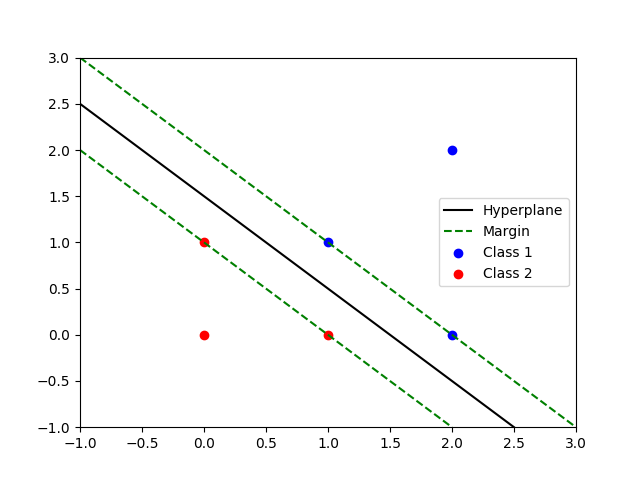
\includegraphics[scale=0.6]{img/hyperplane.png}
\caption{Dibujo del hiperplano óptimo con las dos clases y los márgenes para cada clase.}
\end{figure}

\begin{enumerate}[resume,label=\textit{\alph*})]
	\item ¿Cuáles son los vectores soporte?
\end{enumerate}

\answer

Los vectores soporte son los siguientes:

\begin{itemize}[label=\textbullet]
	\item Para la \textbf{Clase-1}, los vectores soporte son $(1, 1)$ y $(2, 0)$.
	\item Para la \textbf{Clase-2}, los vectores soporte son $(0, 1)$ y $(1, 0)$.
\end{itemize}

\begin{enumerate}[resume,label=\textit{\alph*})]
	\item Construir la solución en el espacio dual. Comparar la solución con la del apartado (a)
\end{enumerate}

\answer



\section*{Ejercicio 4}
\addtoc{Ejercicio 4}

\noindent ¿Cúal es el criterio de optimalidad en la construcción de un árbol? Analice un clasificador
en árbol en términos de sesgo y varianza. ¿Que estrategia de mejora propondría?

\answer

En un principio, el árbol óptimo és el árbol más pequeño capaz de clasificar correctamente todas las instancias. Sin embargo,
intentar obtener este árbol representa un problema NP-completo, con lo cuál computacionalmente es inviable intentar obtenerlo
y hay que intentar utilizar otras técnicas para intentar conseguir árboles subóptimos. Para intentar aprender estos árboles,
podemos utilizar técnicas basadas en heurísticas greedy, las cuáles han demostrado ofrecer unos buenos resultados en general.
La construcción de árboles de esta forma es muy simple: para cada variable, se obtiene la forma en la que esa variable particiona
los datos en clases y se escoge la mejor variable según un determinado criterio. Esa variable forma un nuevo nodo e indica que para
decidir sobre la clase a la que pertenece una instancia, se va a preguntar sobre su valor. Esto se hace de forma recursiva hasta que
no queden más instancias que clasificar.

Existen distintas métricas que se puden utilizar para ver cómo de bien una variable divide un conjunto de datos. Una de ellas
son por ejemplo la \textbf{entropía}, que mide el desorden o falta de información en un nodo, lo cuál significa que cuanto más
equilibradas estén las clases en un conjunto de datos (que las proporciones de datos que pertenecen a una u otra clase sean más o
menos las mismas) significa que hay una entropía alta, y por tanto, no se tiene mucha información, ya las dos clases son casi
equiprobables o están muy cerca de serlo. Existen otras medidas también, como el \textbf{índice de Gini} y el \textbf{error de
clasificación}, las cuáles se utilizan en algunos algoritmos de aprendizaje. Sin embargo, la que nos interesa es la entropía,
ya que uno de los algoritmos más importantes, el \textbf{ID3} utiliza esta métrica. Más concretamente, utiliza la \textbf{ganancia
de información}, que es el concepto opuesto a la entropía.

La idea básica del \textbf{ID3} es escoger aquellas variables que maximicen la ganancia de información. Es decir, queremos
que la variable separe los datos restantes en conjuntos que tengan una entropía lo más pequeña posible, y que por tanto, la mayoría o
todos los elementos de ese conjunto sean de la misma clase (con lo cuál habrá más orden). Así que, para eso, se van escogiendo
aquellos atributos que ofrezcan una mayor ganancia de información y se va construyendo el árbol, de forma que si en alguno de los
conjuntos solo quedan elementos de una clase se crea un nodo hoja con la etiqueta de esa clase. Esto se hace de forma recursiva hasta
que no queden ejemplos por clasificar; es decir, se repite el proceso de escoger una variable con la mayor ganancia de información
y ver como se distribuyen posteriormente los datos. Si se da que quedan ejemplos por clasificar pero no quedan atributos, se escoge
la clase mayoritaria en ese nodo.

Analizando un árbol con los valores de sesgo y varianza, podemos ver que los árboles van a presentar en general un \textbf{sesgo
bajo}, ya que no están asumiendo nada o casi nada sobre la función objetivo, con lo cuál son capaces de aprender casi cualquier
función que se desee a diferencia de otros modelos como por ejemplo los lineales, los cuáles sí que imponen restricciones sobre la
función objetivo (que esta sea lineal). Sin embargo, los árboles suelen presentar una \textbf{alta varianza} debido a que entrenarlos
con una muestra de datos o con otra nos produciría modelos muy diferentes (los nodos y las hojas podrían ser completamente
diferentes).

Debido a que existe una alta varianza en este modelo, podemos intentar disminuirlo a costa de aumentar un poco el sesgo, lo cuál se
conoce como el \textit{bias-variance trade-off}. Para realizarlo, lo que se suele hacer es podar el árbol, eliminando aquellos nodos
que no son muy informativos. Con esto, además, se consigue hacer que el tamaño del árbol se vea reducido efectivamente. Esta poda
puede realizarse mientras se construye el árbol o una vez construido, comprobando el error que se obtiene de validación cruzada. En
el primer caso, se comprueba como va disminuyendo el error a medida que se crea el árbol, y si se da el caso de que en un momento
disminuye muy poco, se deja de construir (lo cuál es conocido como \textbf{early stopping}). En el otro caso, a partir del árbol
construido, se quita cada vez el nodo del árbol que más mejore la precisión con el conjunto de validación hasta que la precisión
que se obtiene sobre este conjunto empiece a empeorar. Esta segunda técnica también es conocida como \textbf{post-prunnning}.

\section*{Ejercicio 5}
\addtoc{Ejercicio 5}

\noindent ¿Cómo influye la dimensión del vector de entrada en los modelos: SVM, RF, Boosting y
NN?

\answer

\section*{Ejercicio 6}
\addtoc{Ejercicio 6}

\noindent El método de Boosting representa una forma alternativa en la búsqueda del mejor clasificador
respecto del enfoque tradicional implementado por los algoritmos PLA, SVM, NN, etc. a)
Identifique de forma clara y concisa las novedades del enfoque; b) Diga las razones profundas
por las que la técnica funciona produciendo buenos ajustes (no ponga el algoritmo); c)
Identifique sus principales debilidades; d) ¿Cuál es su capacidad de generalización comparado
con SVM?

\answer

\section*{Ejercicio 7}
\addtoc{Ejercicio 7}

\noindent Discuta pros y contras de los clasificadores SVM y Random Forest (RF). Considera que
SVM por su construcción a través de un problema de optimización debería ser un mejor
clasificador que RF. Justificar las respuestas.

\answer

\section*{Ejercicio 8}
\addtoc{Ejercicio 8}

\noindent ¿Cuál es a su criterio lo que permite a clasificadores como Random Forest basados en
un conjunto de clasificadores simples aprender de forma más eficiente? ¿Cuales son las
mejoras que introduce frente a los clasificadores simples? ¿Es Random Forest óptimo en
algún sentido? Justifique con precisión las contestaciones.

\answer

\section*{Ejercicio 9}
\addtoc{Ejercicio 9}

\noindent En un experimento para determinar la distribución del tamaño de los peces en un lago, se
decide echar una red para capturar una muestra representativa. Así se hace y se obtiene
una muestra suficientemente grande de la que se pueden obtener conclusiones estadísticas
sobre los peces del lago. Se obtiene la distribución de peces por tamaño y se entregan las
conclusiones. Discuta si las conclusiones obtenidas servirán para el objetivo que se persigue
e identifique si hay algo que lo impida.

\answer

\section*{Ejercicio 10}
\addtoc{Ejercicio 10}

\noindent Identifique que pasos daría y en que orden para conseguir con el menor esfuerzo posible un
buen modelo de red neuronal a partir una muestra de datos. Justifique los pasos propuestos,
el orden de los mismos y argumente que son adecuados para conseguir un buen óptimo.
Considere que tiene suficientes datos tanto para el ajuste como para el test.

\answer

\newpage

\begin{thebibliography}{5}

\bibitem{dlt}
Wikipedia. \textit{Decision Tree Learning}
\\\url{https://en.wikipedia.org/wiki/Decision_tree_learning}

\bibitem{bias-variance}
Jason Brownlee. \textit{Gentle Introduction to the Bias-Variance Trade-Off in Machine Learning}
\\\url{https://machinelearningmastery.com/gentle-introduction-to-the-bias-variance-trade-off-in-machine-learning/}

\bibitem{prunning}
DISPLAYR. \textit{Machine Learning: Pruning Decision Trees}
\\\url{https://www.displayr.com/machine-learning-pruning-decision-trees/}

\end{thebibliography}

\end{document}

